\chapter{Ratchets and Rectification Mechanisms}
\label{ch:ratchetsandrectificationmechanisms}

\section{The Feynman-Smoluchowski ratchet}

The inherent randomness of Brownian motion naturally leads to the question: can this disorder be transformed into order? In other words, can the random thermal motion of particles be used to produce directed movement or extract work? This question sits at the core of statistical mechanics and was famously explored by Richard Feynman in his lectures on physics, through a thought experiment known as the Feynman ratchet and pawl~\cite{feynman1963feynman}.

The Feynman ratchet consists of a set of vanes connected to a ratchet wheel, immersed in a fluid (Fig.~\ref{fig:feynmanratchet}). The idea is: random collisions from the surrounding molecules could push the vanes, but the pawl only allows rotation in one direction. At first glance, this asymmetric mechanism seems capable of converting random thermal motion into unidirectional rotation, apparently violating the second law of thermodynamics.
\begin{figure}
  \begin{center}
    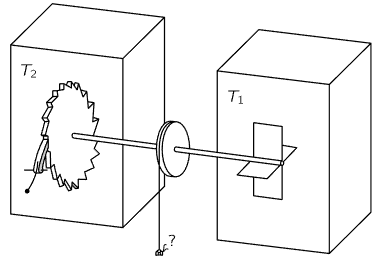
\includegraphics[width=0.65\textwidth]{figures/feynmanratchet.png}
  \end{center}
  \caption[Feynman ratchet]{Visual representation of the Feynman ratchet. Obtained from \cite{feynman1963feynman}}\label{fig:feynmanratchet}
\end{figure}


However, Feynman's analysis showed that when both the ratchet and the pawl are in thermal equilibrium with the same heat bath, the system cannot produce net work. The pawl itself undergoes thermal fluctuations and can occasionally lift off, allowing the ratchet to move backward. Over time, the forward and backward movements average out, and no net rotation occurs. This result reinforces the principle that thermal fluctuations alone cannot be rectified to perform work without a temperature gradient or an external energy input.

\begin{table}[ht]
\centering
\renewcommand{\arraystretch}{1.4}
\caption[Summary of operation of ratchet and pawl.]{Summary of operation of ratchet and pawl. Obtained from \cite{feynman1963feynman}}
\label{tab:ratchet_pawl}
\begin{tabular}{>{\itshape}l l l}
\toprule
\textbf{Forward:} & Needs energy & $\epsilon + L \theta$ from vane. \quad $\therefore$ Rate = $\dfrac{1}{\tau} e^{-(L\theta + \epsilon)/kT_1}$ \\
                  & Takes from vane & $L\theta + \epsilon$ \\
                  & Does work & $L\theta$ \\
                  & Gives to ratchet & $\epsilon$ \\
\midrule
\textbf{Backward:} & Needs energy & $\epsilon$ for pawl. \quad $\therefore$ Rate = $\dfrac{1}{\tau} e^{-\epsilon/kT_2}$ \\
                   & Takes from ratchet & $\epsilon$ \\
                   & Releases work & $L\theta$ \\
                   & Gives to vane & $L\theta + \epsilon$ \\
\bottomrule
\end{tabular}

\vspace{1em}
If system is reversible, rates are equal, hence 
\[
\frac{\epsilon + L\theta}{T_1} = \frac{\epsilon}{T_2}.
\]
\[
\frac{\text{Heat to ratchet}}{\text{Heat from vane}} = \frac{\epsilon}{L\theta + \epsilon}.
\quad \text{Hence} \quad \frac{Q_2}{Q_1} = \frac{T_2}{T_1}.
\]
\end{table}

Despite this limitation, the Feynman ratchet introduced a powerful concept: asymmetry combined with non-equilibrium conditions can, in principle, produce directed motion. This idea is foundational in the study of Brownian motors, biomolecular machines, and active matter systems, including the systems explored in this thesis. In such systems, energy is continuously supplied, whether through bacterial metabolism or magnetic field modulation, creating the necessary non-equilibrium environment that allows motion rectification to occur.

The failure of the Feynman ratchet in thermal equilibrium is intimately connected to another famous thought experiment: Maxwell's demon. Both systems attempt to extract work from thermal fluctuations through selective processes—the ratchet through mechanical asymmetry, and the demon through information gathering.

Maxwell's demon, proposed in 1867, imagines a microscopic being that can sort fast and slow molecules between two chambers, creating a temperature difference without apparent work. Similarly, the pawl in Feynman's ratchet acts as a mechanical "demon," attempting to select only forward fluctuations while blocking backward motion. However, both fail for the same fundamental reason: the cost of selection itself~\cite{maxwell1871theory, maxwell1867letter}.

Brillouin (1951) and later Landauer (1961) showed that Maxwell's demon must expend energy to measure molecular velocities and erase information, with the minimum energy cost being $kT\ln{2}$ per bit erased. In the Feynman ratchet, the pawl must "decide" whether to allow motion, and this decision-making process—manifested as thermal fluctuations of the pawl itself—has an entropic cost that exactly cancels any work extracted~\cite{brillouin1951maxwell, landauer1961irreversibility}.

This connection reveals a deep principle: rectification requires either an information gradient (knowledge about the system) or an energy gradient (non-equilibrium conditions). As Parrondo and Español (1996) demonstrated, the Feynman ratchet can be viewed as an information engine where the pawl performs measurements on the ratchet's position. When the pawl and ratchet are at the same temperature, the information gained equals the entropy produced, yielding no net work~\cite{parrondo1996criticism}.


\section{Brownian ratchets}
\label{sct:brownianratchets}

While Feynman's ratchet fails due to thermal equilibrium, rectified motion becomes possible when detailed balance is broken through external driving. Magnasco (1993) demonstrated this principle through the "rocking ratchet" mechanism~\cite{magnasco1993forced}. In his model, a Brownian particle moves in an asymmetric periodic potential—essentially a sawtooth-shaped energy landscape with gentle slopes in one direction and steep walls in the other.
The crucial innovation was applying an oscillating force $F(t) = A\cos(\omega t)$ that rocks the potential back and forth. Although this force has zero time average—pushing equally left and right—the combination with the spatial asymmetry produces net directional motion. When the force tilts the potential forward, particles easily climb the gentle slopes and can overcome barriers. When tilted backward, particles encounter steep walls and remain trapped. This asymmetric response to symmetric driving breaks the forward-backward symmetry of thermal diffusion.

This mechanism differs fundamentally from Feynman's original ratchet: rather than attempting to rectify equilibrium fluctuations (which violates the second law), the rocking ratchet continuously injects energy through the oscillating force. The time-dependent driving maintains the system far from equilibrium, enabling the spatial asymmetry to generate directed transport. This principle—that asymmetry plus non-equilibrium driving yields rectification—underlies numerous biological processes and provides the theoretical foundation for the magnetically-driven ratchets explored in this thesis.

\begin{figure}[h]
  \begin{center}
    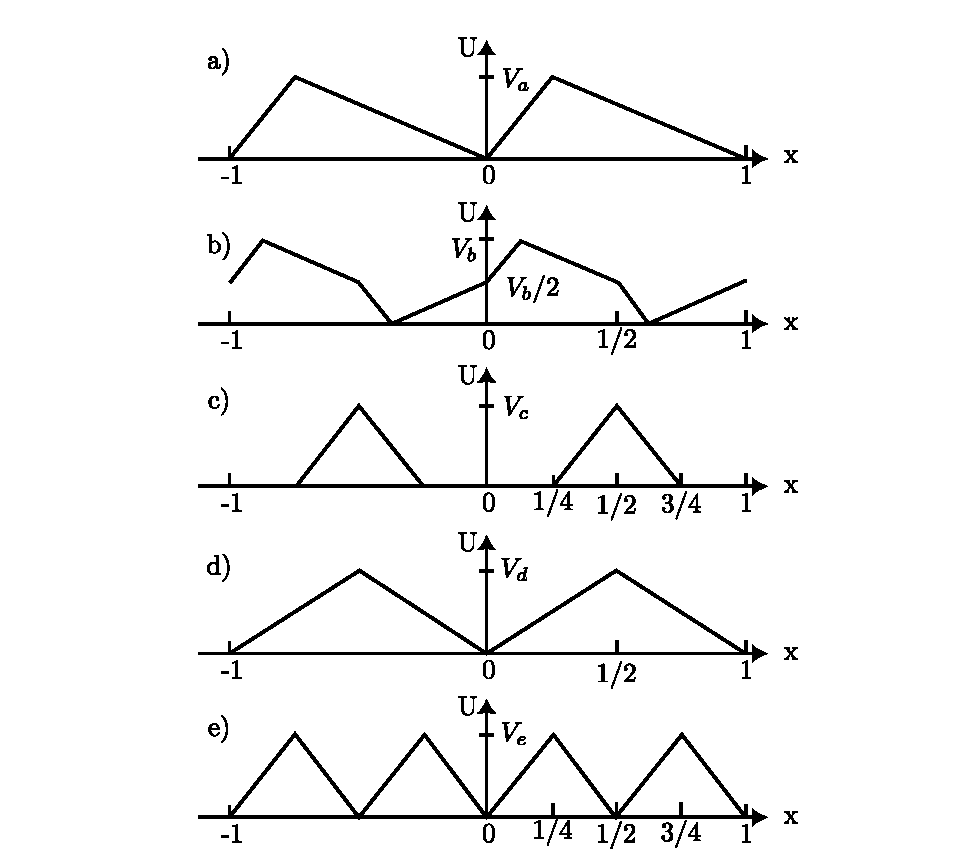
\includegraphics[width=0.95\textwidth]{figures/ratchetpotentialexample.pdf}
  \end{center}
  \caption[Ratchet potential examples.]{Example of ratchet potentials. \textbf{Panel a) and b)} show asymmetric potentials, the remaining are symetric. }\label{fig:ratchetpotential} %%% Paper thermal ratchets with symmetric potentials
\end{figure}


Following Magnasco's rocking ratchet where an oscillating force drives particles in a static potential, Ajdari et al. (1994) analyzed rectification in periodic structures with either spatial or temporal asymmetry~\cite{ajdari1994rectified}. Using a sawtooth potential with asymmetric slopes (steep of height $\epsilon/a$ and gentle of $\epsilon/b$), they identified distinct transport regimes as a function of the AC force amplitude $\gamma$. 

For small forces $\gamma < \epsilon/a$, particles remain trapped. In the intermediate regime $\epsilon/a < \gamma < \epsilon/b$, rectification occurs as particles can climb the gentle slope but not the steep one, yielding either integer velocities $V = n$ when particles fully relax between cycles, or rational velocities $V = n - 1/(m+1)$ when incomplete relaxation creates a periodic pattern over multiple cycles.


This concept was later demonstrated experimentally by Faucheux et al. (1995), who created an "optical thermal ratchet" using focused laser beams~\cite{faucheux1995optical}. To generate a circular trap without introducing external forces, they passed the laser through a plate to create circular polarization, maintaining constant laser intensity along the circular path. By rotating the laser frequency fast enough, particles could not experience any directed force from the beam itself, allowing them to move freely, then modulated the beam intensity to create an asymmetric potential mimicking a ratchet shape, as shown in Figure~\ref{fig:rockingratchets} panel b). They observed that particles localized in potential minima when the modulation was turned on, while for sufficiently long periods, particles moved either backward or forward with equal probability.


A different approach was developed by Lee et al. (2004), who employed holographic optical trapping with a symmetric potential~\cite{lee2005observation}. Their system consisted of discrete optical tweezers functioning as potential wells. Between each state, particles are released and free to diffuse, nevertheless they can rapidly jump between adjacent traps. Using this methodology, they achieved net particle displacement in one direction, as illustrated in Figure~\ref{fig:rockingratchets}. Remarkably, when they reversed the direction of well displacement, particles followed the trap movement in the opposite direction. Due to this predictable response to trap motion, they named this system a "deterministic thermal ratchet."

\begin{figure}
  \begin{center}
    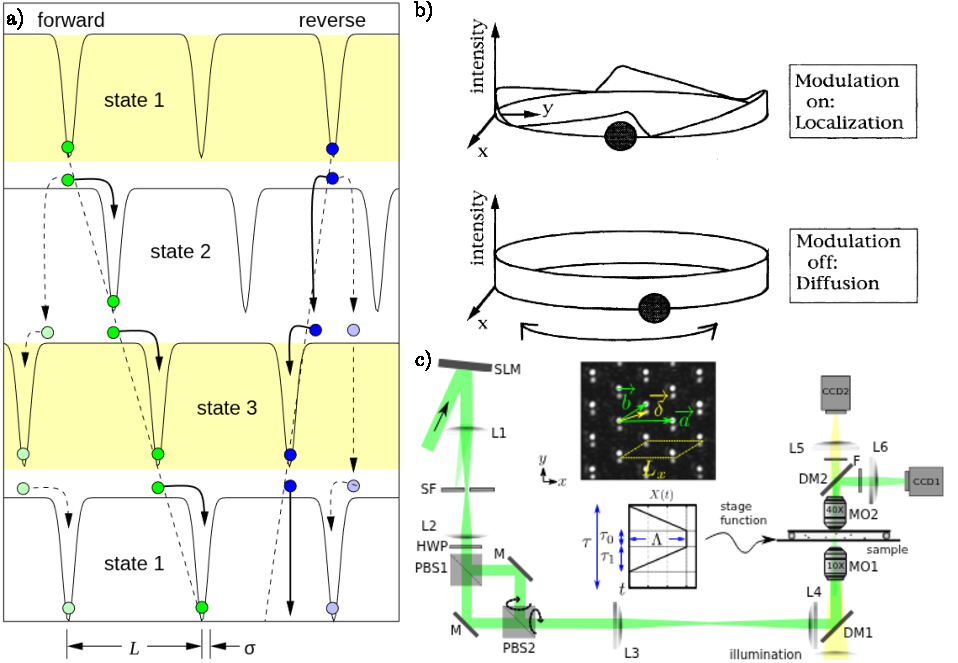
\includegraphics[width=0.95\textwidth]{figures/rockingratchets.pdf}
  \end{center}
  \caption[Rocking ratchets expermients.]{\textbf{Panel a)} Discrete pattern of optical traps with displacement in one directio, minimum width of $\sigma$ and a maximum width of $L$. Obtained from~\cite{lee2005observation}. \textbf{Panel b)} When the modulation is on, the beam intensity follows the shape of a ratchet potential with 4 periods per cycle. When the modulation is off, the intensity remains constant, allowing particles to diffuse freely. Obtained from~\cite{faucheux1995optical}. \textbf{Panel c)} Experimental setup of the spatial light modulator, upper inset shows the basis vectors ($\vec{a}$ and $\vec{b}$) of the main lattice and the displacement for the clone lattice ($\vec{delta}$), the lower inset illustrates the movement amplitude of the stage, obtained from~\cite{arzola2017omnidirectional}}\label{fig:rockingratchets}
\end{figure}



 Lebedev et al. (2009) modified this approach by using three linearly polarized beams acting only in the xy-plane, as shown in Figure~\ref{fig:lebedevexperiment}~\cite{lebedev2009two}. They applied forces to particles by phase-modulating two of the three lasers, which shifts the entire optical lattice. The modulation was generated using RF generators to produce potentials $V_x$ and $V_y$. The sum $V_x + V_y$ served as the input signal for beam 2, while the difference $V_x - V_y$ was used for beam 3, creating the rocking forces. They studied this system using ultracold rubidium atoms as test particles. To track the atomic positions, they employed a CCD camera to determine the center of mass of the atomic cloud.

 In their first experiment, they applied a biharmonic drive along only one axis. As expected, the system reduced to a one-dimensional harmonic ratchet, and they observed directed particle motion along the axis of the applied biharmonic force. In subsequent experiments, they applied harmonic drives along both axes, with one frequency being twice the other. Their results showed that particles experienced directed motion along the axis with the faster harmonic, while motion along the other axis remained diffusive. In their final experiment, they applied biharmonic drives simultaneously along both axes to investigate whether directed transport could be achieved in two dimensions. By varying the relative weights of the forces along each axis, they demonstrated that it was possible to control the atomic displacement and direct atoms to specific target positions as shown in Figure~\ref{fig:lebedevexperiment} a).


 \begin{figure}[h]
  \begin{center}
    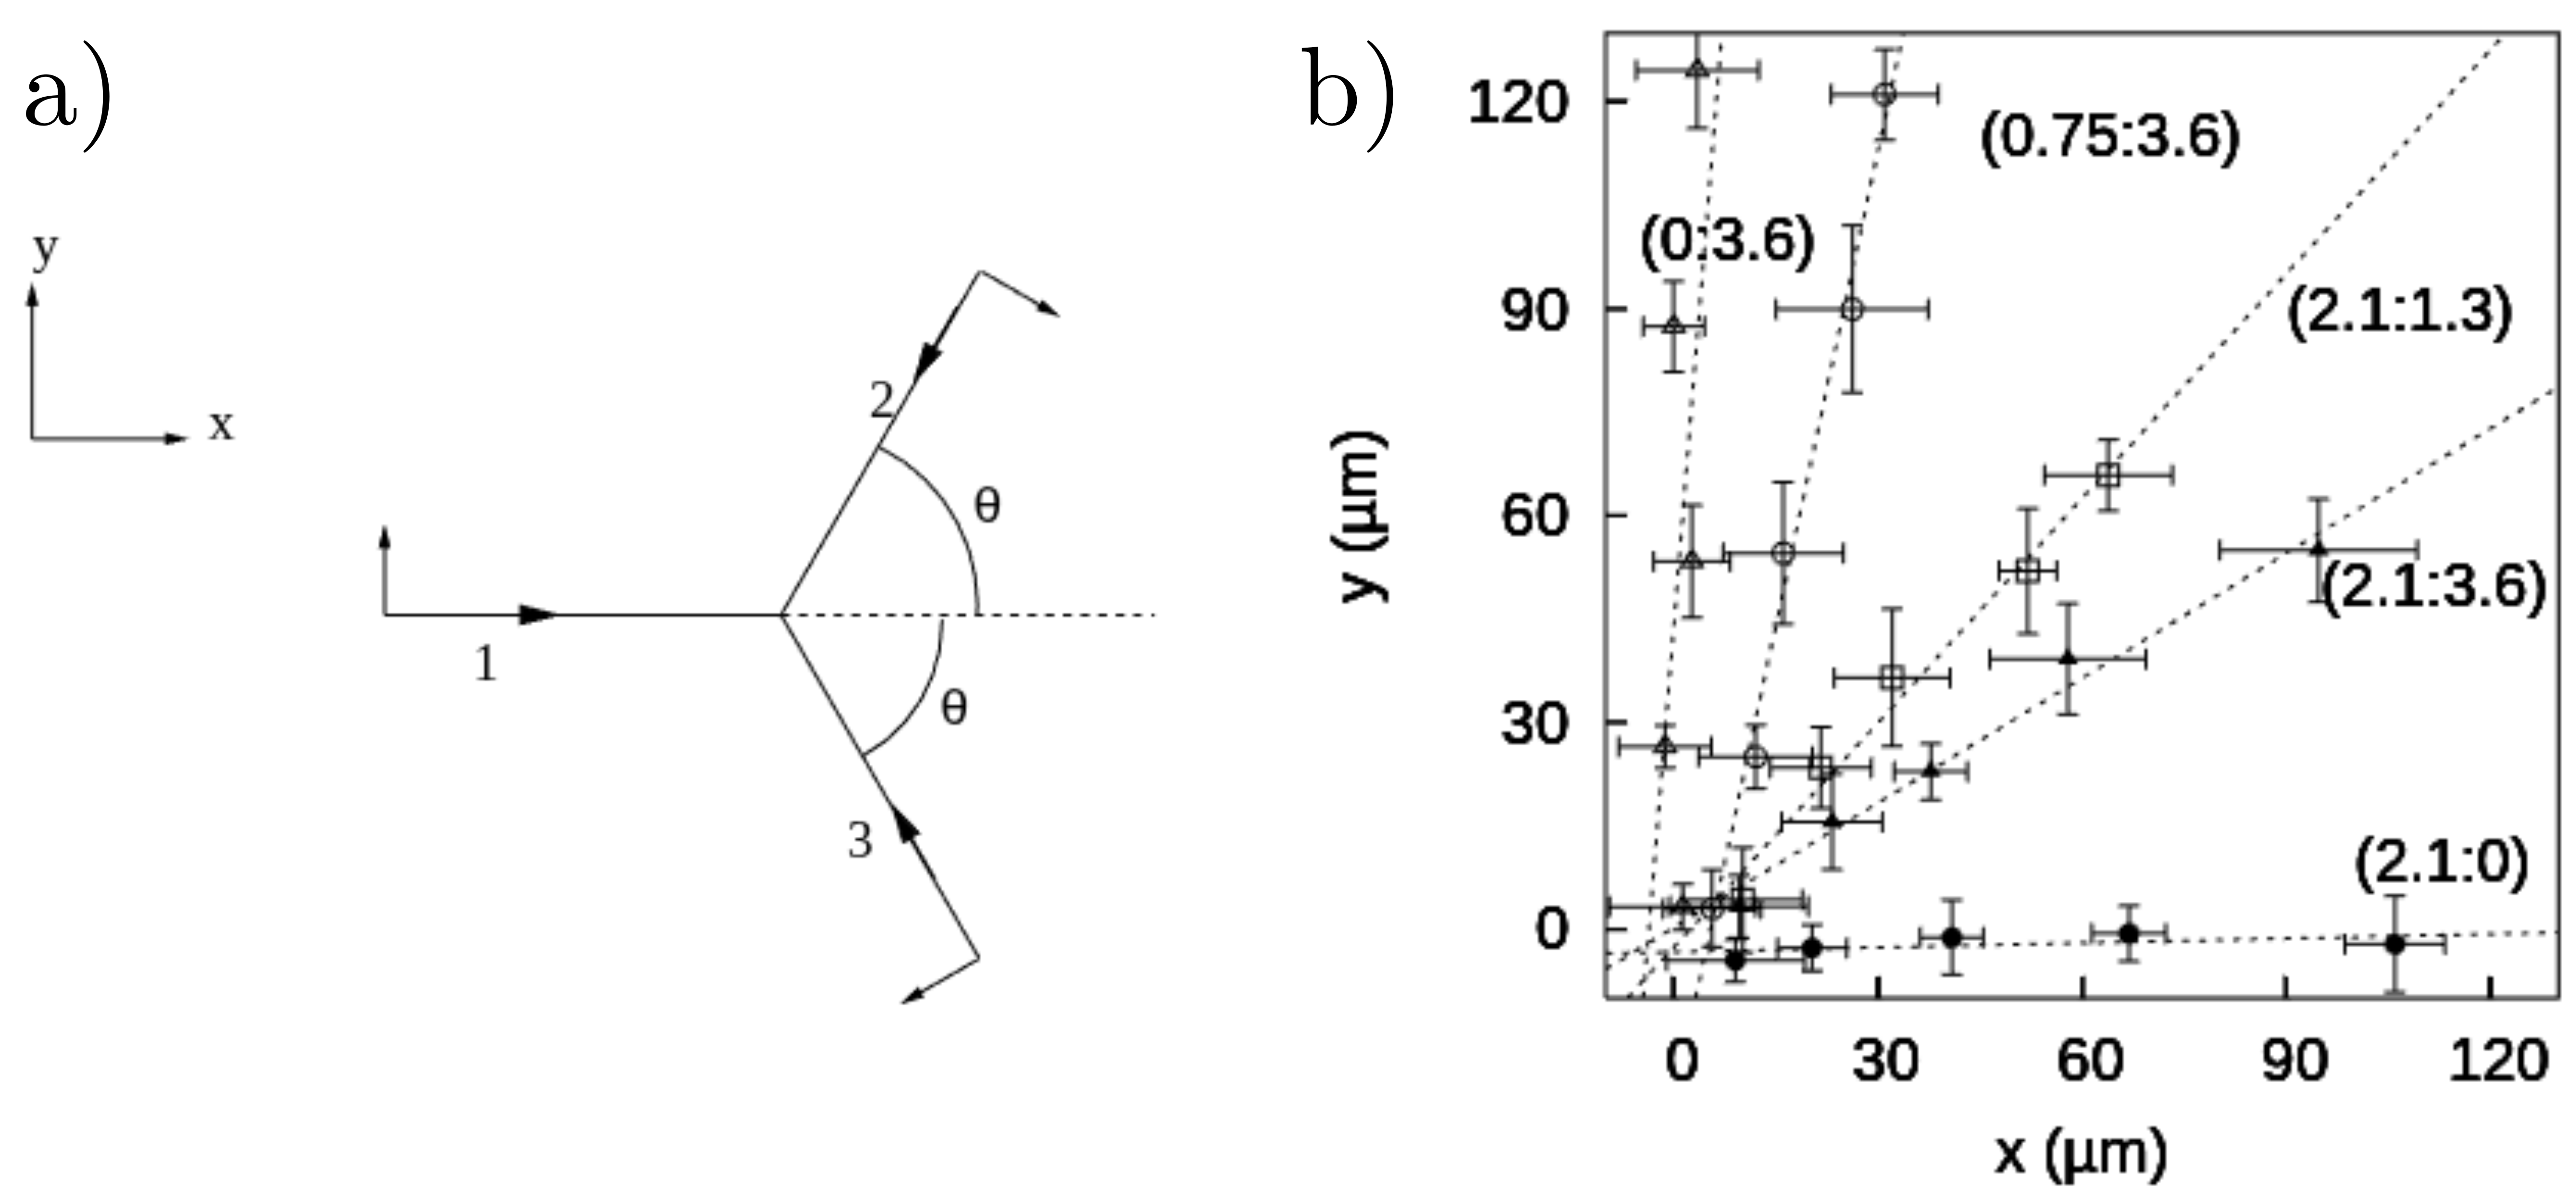
\includegraphics[width=0.80\textwidth]{figures/LebedevExperiment.png}
  \end{center}
  \caption[Lebedev experiment.]{\textbf{Panel a)} Lattice beam configuration in the xy plane. $\theta$ = 60°. \textbf{Panel b)} Position of the atomic cloud center of mass at different instants and forces when applying biharmonic at ehe same time in xy-plane. Obtained from~\cite{lebedev2009two}.}\label{fig:lebedevexperiment}
 \end{figure}


 Following the same lattice-based approach, Arzola et al. (2017) successfully recreated all five two-dimensional Bravais lattices using computer-generated holographic optical micromanipulation~\cite{arzola2017omnidirectional}. Their potential consisted of Gaussian wells distributed along a primary lattice, combined with a shifted replica of the same lattice with a reduced depth factor, Q, compared to the original. The asymmetry of the resulting potential depended directly on both the depth factor Q and the displacement between the original and replica lattices. They implemented the rocking mechanism by moving the particle cell along one axis.

The researchers performed three main experiments to validate their results, each with three different diffusion parameters (including no diffusion as one condition), calculating the current in the x and y axes with respect to the amplitude of movement. In the first experiment, they set the asymmetry parallel to the rocking force. They observed that since the wells were aligned with the particle movement, particles tended to move in the direction of the force, traveling from well to well, while experiencing no movement in the perpendicular direction. Current was present along the entire amplitude range.

The second experiment positioned the asymmetry perpendicular to the rocking force direction, yielding interesting results. Similar to the first experiment, current appeared along only one axis (the asymmetry axis), but the current behaved like a Gaussian bell curve. When the rocking movement amplitude approached the asymmetry lattice spacing, particles only moved back and forth between two wells in the x direction, experiencing no current in the y axis.

For the final experiment, they examined how the system behaved under a combination of both previous configurations. They created an oblique lattice with the asymmetry aligned with the rocking force direction, producing an oblique particle current. The results were essentially a combination of the two previous experiments: at certain amplitudes, current appeared in both axes, but as amplitude increased, the y-axis current decreased while the x-axis current increased. 


Feynman demonstrated that a purely thermal Brownian ratchet cannot generate directed motion due to the second law of thermodynamics. However, introducing specific conditions to break symmetry has proven ideal for bypassing these limitations.

One successful approach to achieving this symmetry breaking involves rocking ratchets, where an external periodic drive is applied to an asymmetric potential. Previous experiments have demonstrated the potential of optics to create such asymmetries with high precision and control. While obtaining directed motion at the microscale remains challenging, by applying these symmetry-breaking parameters it becomes possible not only to overcome thermal noise but to harness it for directional transport. Unfortunately, as shown in previous works, implementing these systems often requires specific and sophisticated experimental setups. Interestingly, nature has already developed an alternative solution by creating matter capable of self-propulsion, known as active matter, which achieves directed motion through entirely different mechanisms.



